\section{The Research Artifacts}

The first artifact consists of two main components: the Clean Architecture Expander and
the Expander framework. The name of the Expander Framework, Pantha Rhei, was inspired by
the Greek philosopher \emph{Heraclitus}, who famously stated that \enquote{life is flux.}
The name reflects the artifact's perceived ability to cope with constant change in a
stable and evolvable manner. Users can interact with the Expander Framework using the
\gls{cli} command \enquote*{flux} in combination with several parameters.

As illustrated in Figure \ref{fig_overview_design}, the main task of the first artifact or
\enquote*{expand} the second artifact. By entering the correct command, the Expander
Framework loads the model being instantiated during the expansion process. Then, the
required expanders are prepared based on information available through the model. In the
case of this study, the Clean Architecture Expander. The Clean Architecture Expander
consists of a set of tasks and templates. When the Expander Framework executes the Clean
Architecture Expander, the model is instantiated into the generated artifact with the aid
of the templates.

The model is an instance of the meta-model. Consequently, the model can represent any
application as long as the meta-model is respected. In the case of this study, the model
represents the entities, attributes, relationships, and other characteristics of the
meta-model.

As a result, the second artifact (artifact II) allows a user to modify or maintain the
model used by the Expander Framework by exposing a Restful interface. This method
approaches the meta-circularity process, where an expansion process is used to update the
meta-model. Although not fully compliant with the theory of \gls{ns}, the Expander
Framework consists of the required tasks to update its own meta-model. This is illustrated
in Figure \ref{fig_overview_design} by the \enquote*{updates} arrow.

\begin{figure}[htbp]
    \centering
    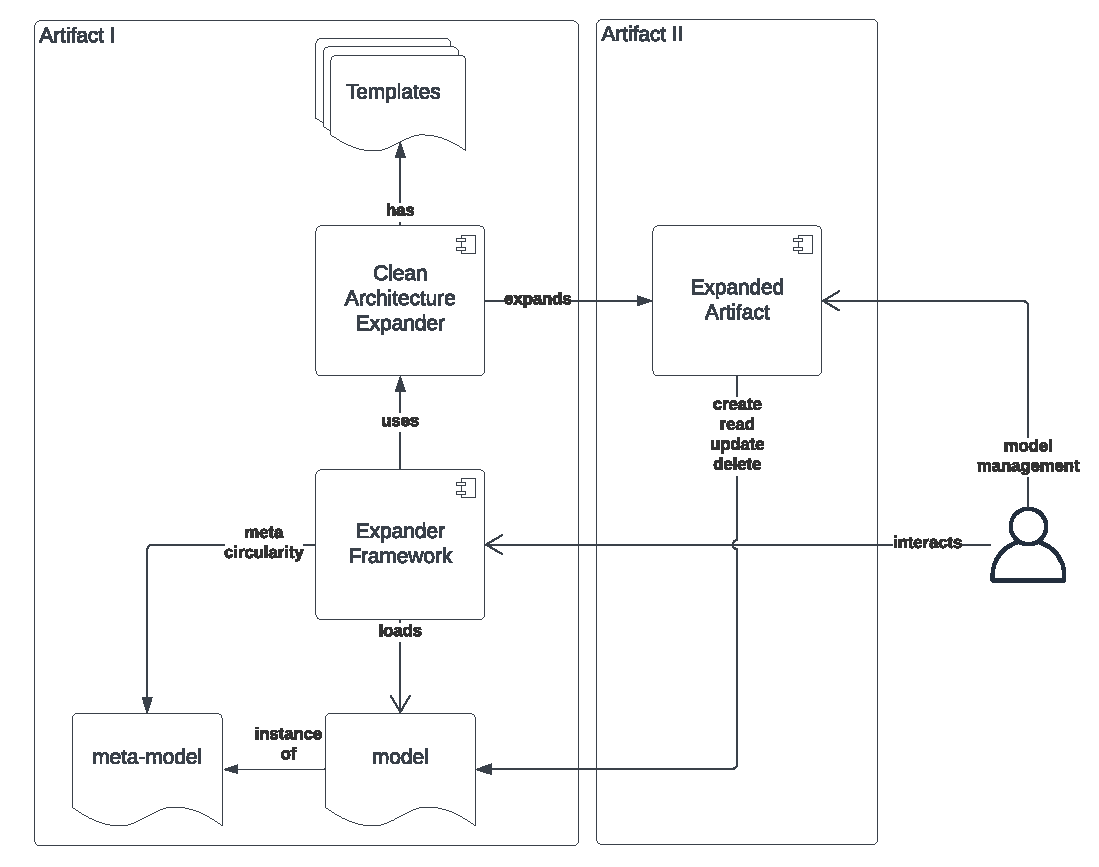
\includegraphics[width=0.4\textwidth]{figures/artifactOverview.pdf}
    \caption[Schematic overview of the artifacts]{Schematic overview of the artifacts}
    \label{fig_overview_design}
  \end{figure}

\input{content/artifacts/name}
\section{The Meta-Model and Model} \label{sec_artifact_meta_model}

The meta-model is a blueprint that describes a software system's structure, entities,
relationships, and expanders. The model is an instantiation of the meta-model,
representing a specific software system with unique characteristics. 

Figure \ref{fig_erd} illustrates the version of the meta-model used for this research. A
detailed description of each of the elements can be found in Appendix
(((REPLACE FULLREF)))

\begin{figure}[htbp]
    \centering
    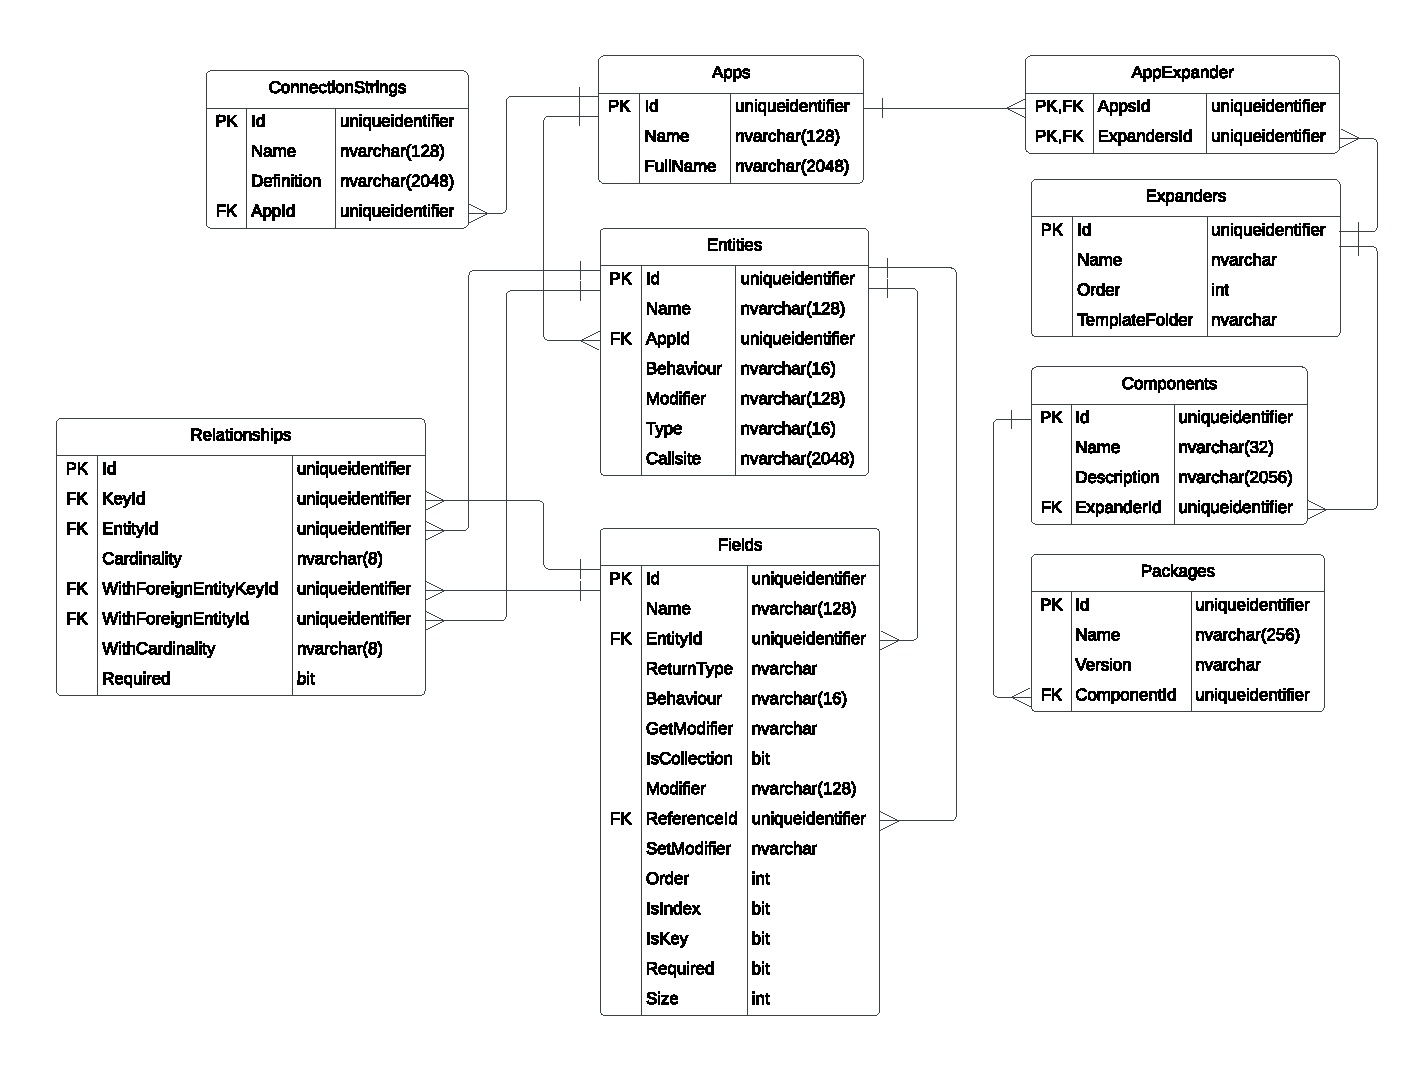
\includegraphics[width=0.4\textwidth]{figures/erd.pdf}
    \caption[The meta-model represented as an Entity Relationship Diagram]{The meta-model represented as an Entity Relationship Diagram}
    \label{fig_erd}
\end{figure}
\section{Plugin Architecture} \label{subsec_plugin_architecture}

The Expander Framework artifact is responsible for loading and bootstrapping Expanders and
initiating the generation process. Expanders are dynamically loaded at runtime through a
dotnet capability called assembly binding, allowing the architecture illustrated in the
following image \parencite{koks_expanderpluginloaderinteractor_2023}.

\begin{figure}[htbp]
  \centering
  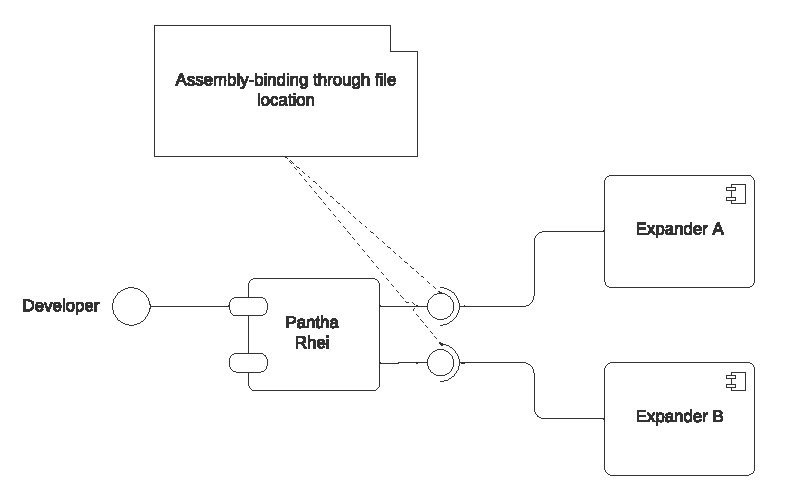
\includegraphics[width=0.4\textwidth]{figures/plugin_architecture.pdf}
  \caption[Plugin Archticture]{Expanders are considered plugins}
  \label{fi:plugin_architecture}
\end{figure}

This plugin design adheres to several principles of \gls{solid}. The \gls{srp} principle
is implemented by ensuring that an expander generates one and only one construct. The
\gls{ocp} principle is applied by allowing the creation of new expanders in addition to
the already existing ones. The \gls{lsp} principle is respected by enabling the addition
or replacement of expanders without modifying the internal workings of the Expander
Framework.
\section{Expanders}

The Exander Framework allows for the miscellaneous execution of expanders of any type. The
Expander Framework is independent of any of the details of Expanders, fully adhering to
the principle of \gls{dip}. Conversely, an Expander is required to implement several
interfaces to ensure execution and dependency management are available during runtime. The
Expander Framework also consists of a set of default tasks, such as the execution of the
expansion tasks known as ExpanderHandlerInteractors
\citecode{koks_iexpanderhandlerinteractor_2023}, logging, bootstrapping dependencies, and
tasks to execute harvestings and injections. Except for the use of the
IExpanderInteractor, non of which are required.

Figure \ref{fig_expander_design} illustrates the dependencies between the domain layer of
the Expander Framework. The Clean Architecture Expander is considered an application layer
containing specific tasks bounded to a particular application or process. In this case,
the Expansion process.

\begin{figure}[htbp]
    \centering
    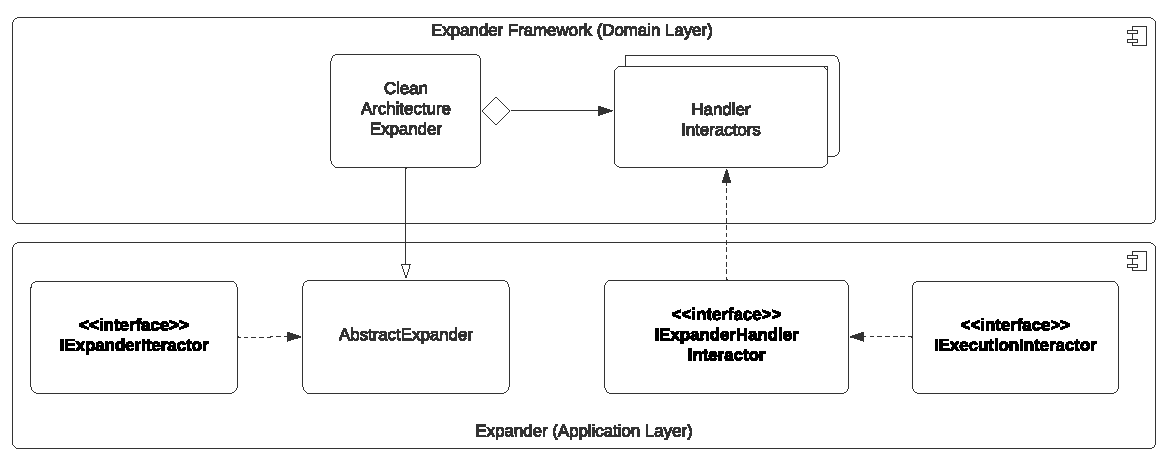
\includegraphics[width=0.4\textwidth]{figures/expander.pdf}
    \caption[The design of an Expander]{The design of an Expander}
    \label{fig_expander_design}
  \end{figure}
\section{Executing Commands} \label{subsec_IExecutionInteractorObject}

An exciting implementation that facilitates a high degree of cohesion while maintaining
low coupling is the utilization of the \code{koks_iexecutioninteractor_2023} interface
\parencite{koks_iexecutioninteractor_2023}. This interface allows for the execution of
various derived types responsible for various tasks, such as executing Handlers,
Harvesters, and Rejuvenators\footnote{It is important to note that the Rejuvenation
objects in this version of the artifact are capable of performing injections and not the
entire Rejuvenation process.} \parencites{koks_expandentitieshandlerinteractor_2023,
koks_regionharvesterinteractor_2023, koks_regionrejuvenatorinteractor_2023}. The
implementation promotes decoupling by adhering to both \gls{ocp} and \gls{lsp}.

\begin{figure}[htbp]
    \centering
    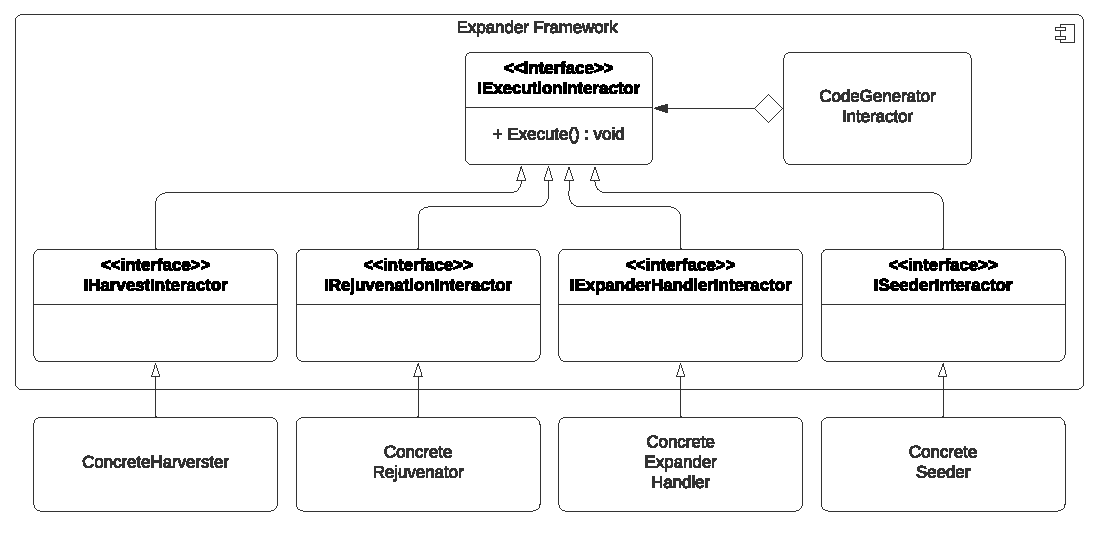
\includegraphics[width=0.4\textwidth]{figures/command_pattern.pdf}
    \caption[Low coupling with \code{koks_iexecutioninteractor_2023}]{Low coupling with \code{koks_iexecutioninteractor_2023}}
    \label{fig_iexecutioninteractor}
  \end{figure}


Figure \ref{fig_iexecutioninteractor} illustrates that the required interfaces are placed
in the Domain layer of the Expander Framework. In contrast, the concrete classes also can
be implemented as part of the internal scope of the Clean Architecture Expander
\parencite{koks_migrationharvesterinteractor_2023}. Code listing
(((REPLACE CODE LISTING))) illustrates an implementation example of
this interface. Finally, the code listing (((REPLACE CODE LISTING)))
illustrates the aggregation of the execution, which allows for a graceful cohesion of the
execution Tasks \parencite{koks_codegeneratorinteractor_2023}.

\subsection{Dependency Management}

Dependency management is an extremely valuable aspect of achieving stability and
evolvability. Dependency management can be achieved by using Dependency Injection. This
research acknowledges \textcite[215]{mannaert_normalized_2016} statement that Dependency
Injection does not solve coupling between classes. Working on the artifact has shown that
combinatorial effects can occur when not careful. Nevertheless, Dependency Injection is a
widely used pattern in building the artifact. In order to achieve stability and
evolvability, the Dependency Injection pattern \underline{must} be combined with various
other principles of both \gls{ca} and \gls{ns}. 

The goal is to centralize the management of dependencies and remove unwanted manual object
instantiations in the code. Al this while respecting the \gls{dip} principle so that each
component layer is responsible for managing its dependencies. The artifact achieves this
by using extension methods \parencite{koks_dependencyinjectionextension_2023}. Additionally, and quite significantly,
implementations primarily rely on abstractions or contracts (interfaces) instead of the
details of concrete implementations. 

Traditionally, Dependency Injection injects instantiations through constructor parameters
or class properties. Although there are benefits in this approach, doing so will
eventually lead to combinatorial effects, breaking the stability of a software artifact.
In order to solve this problem, the artifact used the Service Locator pattern, a central
registry responsible for resolving dependencies \parencite{wikipedia_service_2023}. Many
frameworks are available from \gls{nuget}, but the artifact uses the Service Registry,
which is part of the .NET framework. This service registry is considered a cross-cutting
concern. The dependency on this technology is reduced by applying the principles of the
\gls{lsp} and \gls{isp}. The artifact creates and uses separate interfaces to register
\parencite{koks_idependencymanagerinteractor_2023} and resolve
\parencite{koks_idependencyfactoryinteractor_2023} dependencies. The framework technology
dependencies are abstracted behind implementing those interfaces
\parencite{koks_dependencymanagerinteractor_2023}. 

Practically every class gets the \citecode{koks_idependencyfactoryinteractor_2023}
injected, on which further resolving is responsible for that class's inner workings. Code
Listing \ref{list_Injecting} illustrates how this is done in the
\citecode{koks_abstractexpander_2023} class. Finally, all the dependencies are
bootstrapped on application bootup, depicted in Code Listing \ref{list_dip}. 

The approach described here has many advantages in managing the stability and evolvability
of the software artifact. However, as for most things, there are also some drawbacks. For
example, a good amount of experience is required for developers to understand code that
incorporates abstractions, contracts, and Dependency Injection. Another drawback is that
dependency errors are detected in runtime rather than compile time. The benefits of the
artifacts, however, outweigh the drawbacks.